\documentclass[a4paper,10pt]{article}
\usepackage{graphicx}

\title{Proposal: Web Content Extraction Through Machine Learning}
\author{
    Ziyan Zhou \\
    ziyanjoe@stanford.edu
    \and
    Lei Sun \\
    sunlei@stanford.edu
}

\date{\today}

\begin{document}
\maketitle

\section{Motivation and Goal}

Understanding the web is hard. The idea of semantic web, dating back almost to the invention of the web, that the various parts of web pages should be tagged such that machines as well as humans can make inferences based on the information they contain, has never gotten very far. Nowadays, the problem has worsen due to the increased complexity in web technology that came with better human interfaces and more creative designs. Even though various new semantic web technologies have been hyped up again in recent years, for example RSS and Open Graph, there remains the central problem of requiring content to be formatted twice, once for the machines’ benefit and once for the actual humans.

On the other hand, it is trivial for a parser to extract the underlying content of a web page when it is told the structure of the page. But as the number of website increases exponentially, it is hard, even impossible to analyze all websites manually one by one, not to mention that the page structure for a known site could be changing over time.

Fortunately, web pages on the same site often share very similar structures. These pages are usually generated and presented by a content management system with some web templates and a structured data source backend. Humans are intrinsically good at discerning the common structure of these web pages, and with some experience, can quickly locate the relevant content on a complex page without a second glance. See \emph{Figure 1}.

\begin{figure}[htp]
\centering
\includegraphics[scale=0.65]{theverge_labeled}
\caption{Example article with title and content labeled}
\label{}
\end{figure}

Given a set of similar pages from a specific site, the goal of this project is to teach machines to look at web pages the same way as humans would do, to discover the structure of the pages through unsupervised learning and computer vision techniques, and then to extract the vital information while filtering out distractions.


\section{Data Extraction}

For the scope of this project, the training and testing dataset will be extracted from popular English news article sites on the Internet, including theverge.com, npr.org, nytimes.com.

For each site, multiple article pages will be fetched and fully rendered in a virtual webkit browser. Text enclosing blocks will then be identified. See red boxes in \emph{Figure 2}. For each block, a set of features will be extracted, including the size and position of the block, the contained text, the font configuration, color, line height, tag path, etc. For example, an extracted block may contain data similar to the following:

\begin{verbatim}
{
  "bound": {
    "height": 115,
    "left": 385,
    "top": 934,
    "width": 565
  },
  "computed": {
    "color": "rgb(51, 51, 51)",
    "fontFamily": "Helvetica, Arial, sans-serif",
    "fontSize": "14px",
    "fontStyle": "normal",
    "fontWeight": "normal",
    "height": "115px",
    "lineHeight": "23px",
    "opacity": "1",
    "width": "565px"
  },
  "text": [
    "Microsoft has",
    " cut the price",
    " of the Surface RT in recent weeks due to ...",
    "interview with ",
    "CNET",
    ", Nvidia CEO Jen-Hsun Huang has revealed ...",
    ", Huang is hopeful about the upcoming Surface refresh."
  ],
  ...
}
\end{verbatim}

\begin{figure}[htp]
\centering
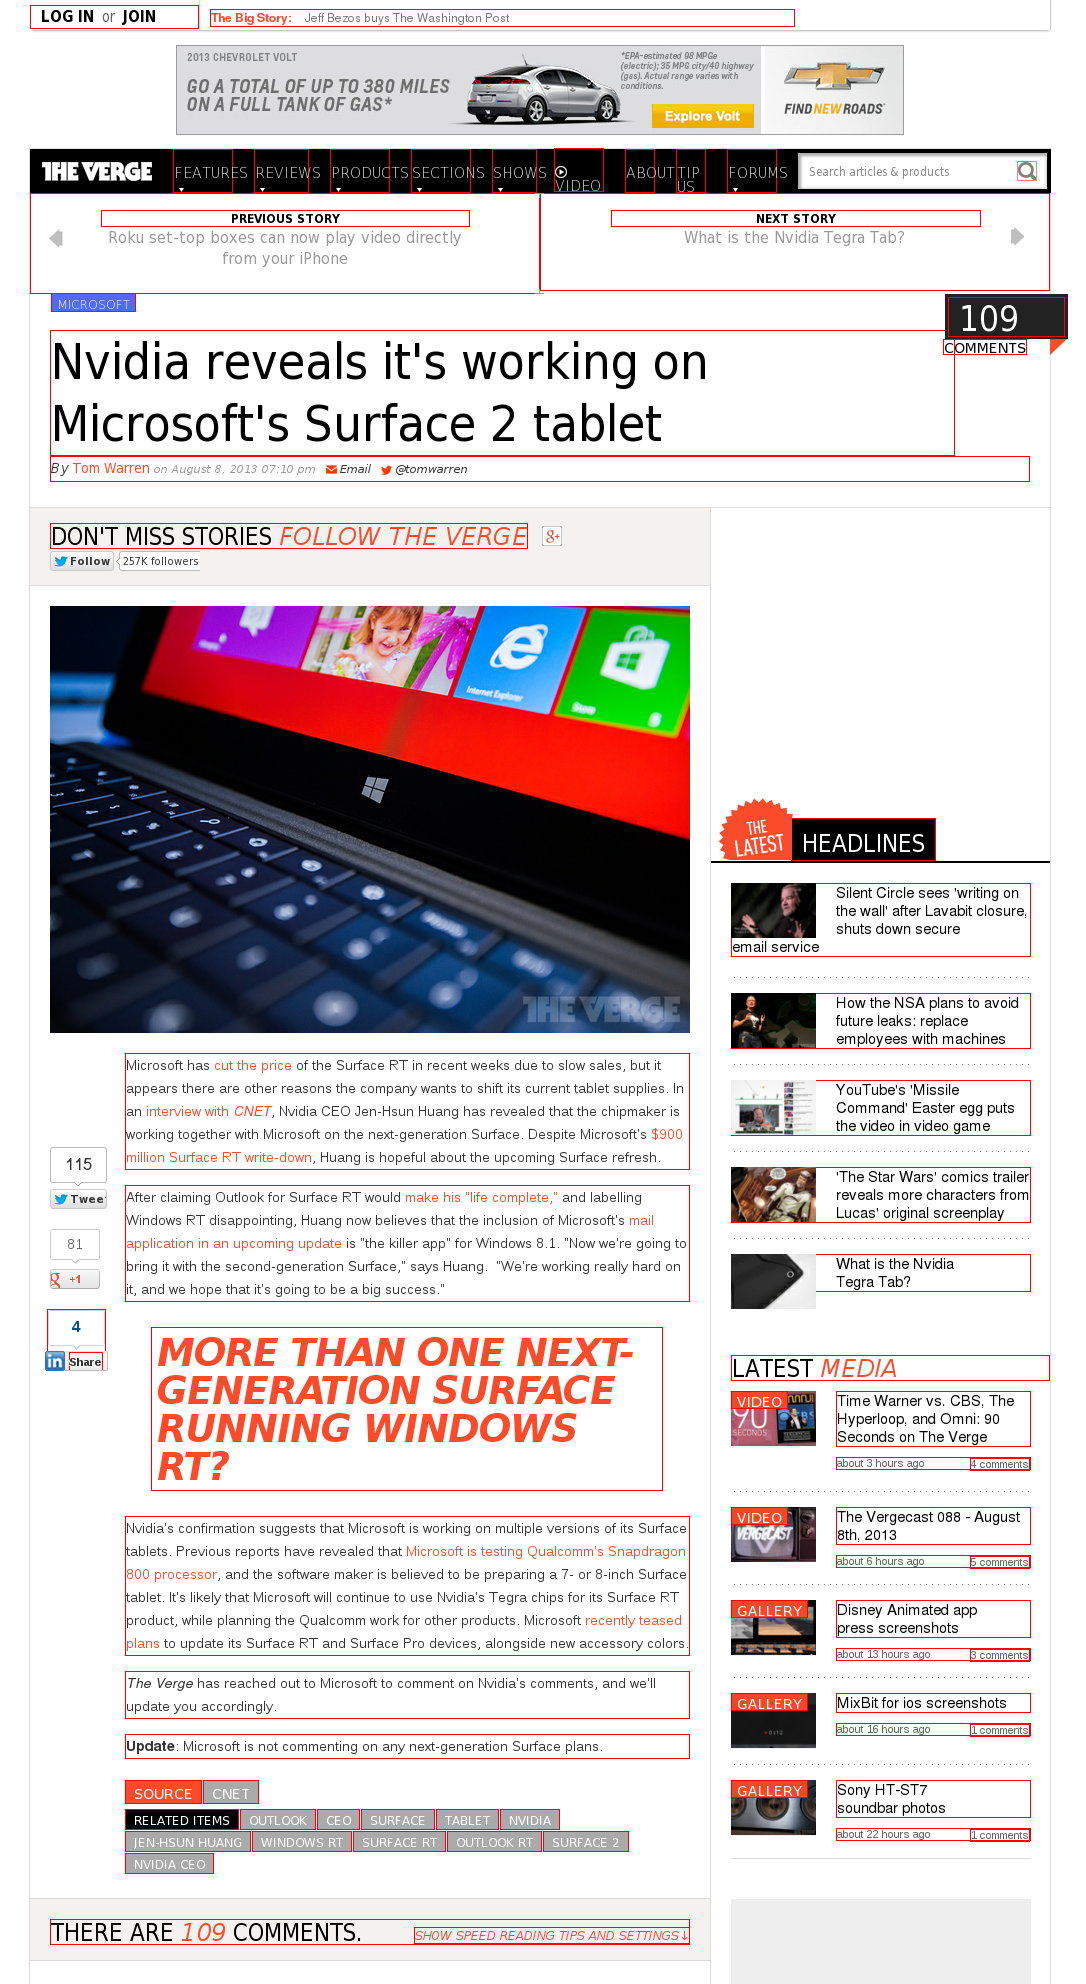
\includegraphics[scale=0.28]{theverge_blocks}
\caption{Text blocks identified as red boxes in example article, rendered by virtual webkit browser}
\label{}
\end{figure}

From the same set of websites, a number of extra article pages with content manually extracted will be used as the testing set to evaluate the performance of the algorithm.


\section{Initial Hypothesis}

Text containing blocks on a page can be clustered based on their features. One of the clusters should contain blocks for the article title. One or more of the clusters should contain relevant blocks from which the entire article content can be reconstructed. The clusters containing the useful blocks can be identified through the help of meta tags on the page, like title and description.


\end{document}
